\documentclass{pretexto/report}
% --- Archivo de bibliografía -----------------
\addbibresource{pretexto/repbib.bib}

\def\fillandplacepagenumber{%
 \par\pagestyle{empty}%
 \vbox to 0pt{\vss}\vfill
 \vbox to 0pt{\baselineskip0pt
   \hbox to\linewidth{\hss}%
   \baselineskip\footskip
   \hbox to\linewidth{%
     \hfil\thepage\hfil}\vss}}


\title{Análisis y diseño}

%%%%%%%%%%%%%%%%%%%% TERMINA PREÁMBULO %%%%%%%%%%%%

\begin{document}

%%%%%%%%%%%%%%%%%%%% PORTADA %%%%%%%%%%%%%%%%%%%%%%%

\begin{titlepage}
  \thispagestyle{empty}
  \pagecolor{white}
  
  % Encabezado con logos
  \begin{center}
    \vspace{1cm}
    
    % Logos en la parte superior
   
      \centering
          \vspace{2cm}
      
\includegraphics[height=2.35cm]{img/logos.png}
    
    \vspace{3cm}
    
    % Tipo de trabajo
    {\normalsize\color{charcoal}\textsc{Tarea}}\\[0.5cm]
    
    % Título principal
    {\huge\bfseries\color{black}Análisis y Diseño de software}\\[0.5cm]

    
    \vspace{1.5cm}
    
    % Información de autores
    {\small\color{charcoal}\textsc{Realizada por}}\\[0.3cm]
    
    {\normalsize\color{black}Robles Guzmán Naomi Isabel}\\[0.2cm]
    {\normalsize\color{black}Ugalde Téllez Aarón}\\[0.5cm]

    
    \vspace{0.8cm}
    
    % Información académica
    {\small\color{charcoal}\textsc{Para la materia de}}\\[0.2cm]
    {\normalsize\color{blue}Ingeniería de Software para Sistemas Inteligentes}\\[0.5cm]
    
    {\small\color{charcoal}\textsc{Impartida por}}\\[0.2cm]
    {\normalsize\color{black}Chadwick Carreto Arellano}\\[0.5cm]
    
    {\small \color{charcoal}\textsc{Grupo}}\\[0.3cm]
    {\normalsize\color{black}6BM1}\\[0.8cm]
    
    \vfill
    
    % Línea decorativa y fecha
    {\color{blue}\rule{0.4\textwidth}{1pt}}\\[0.3cm]
    {\large\color{charcoal}03 de octubre de 2025}
    
    \vspace{1cm}
    
  \end{center}
\end{titlepage}                                                     

%%%%%%%%%%%%%%%%%%%% ÍNDICES %%%%%%%%%%%%%%%%%%%%%%%%%%
\tableofcontents 
\pagebreak


%%%%%%%%%%%%%%%%% INTRODUCCIÓN %%%%%%%%%%%%%%%%%%%%%%%%

\pagebreak
\section{Análisis y Diseño del sistema}

\subsection{Objetivos}

\begin{itemize}
    \item Desarrollar un sistema que permita al usuario registrar sus habitos y tareas diarias
    \item Añadir espacios para que el usuario agregue datos que sirvan de contexto para las recomendaciones inteligentes.
    \item Implementar un modulo que realice recomendaciones inteligentes sobre como realizar los habitos y tareas registradas
    \item Realizar una interfaz intuitiva y atractiva que permita añadir las tareas y habitos de manera facil
\end{itemize}


\subsection{Diagrama de Entradas y Salidas}

\begin{figure}[H]
    \centering
    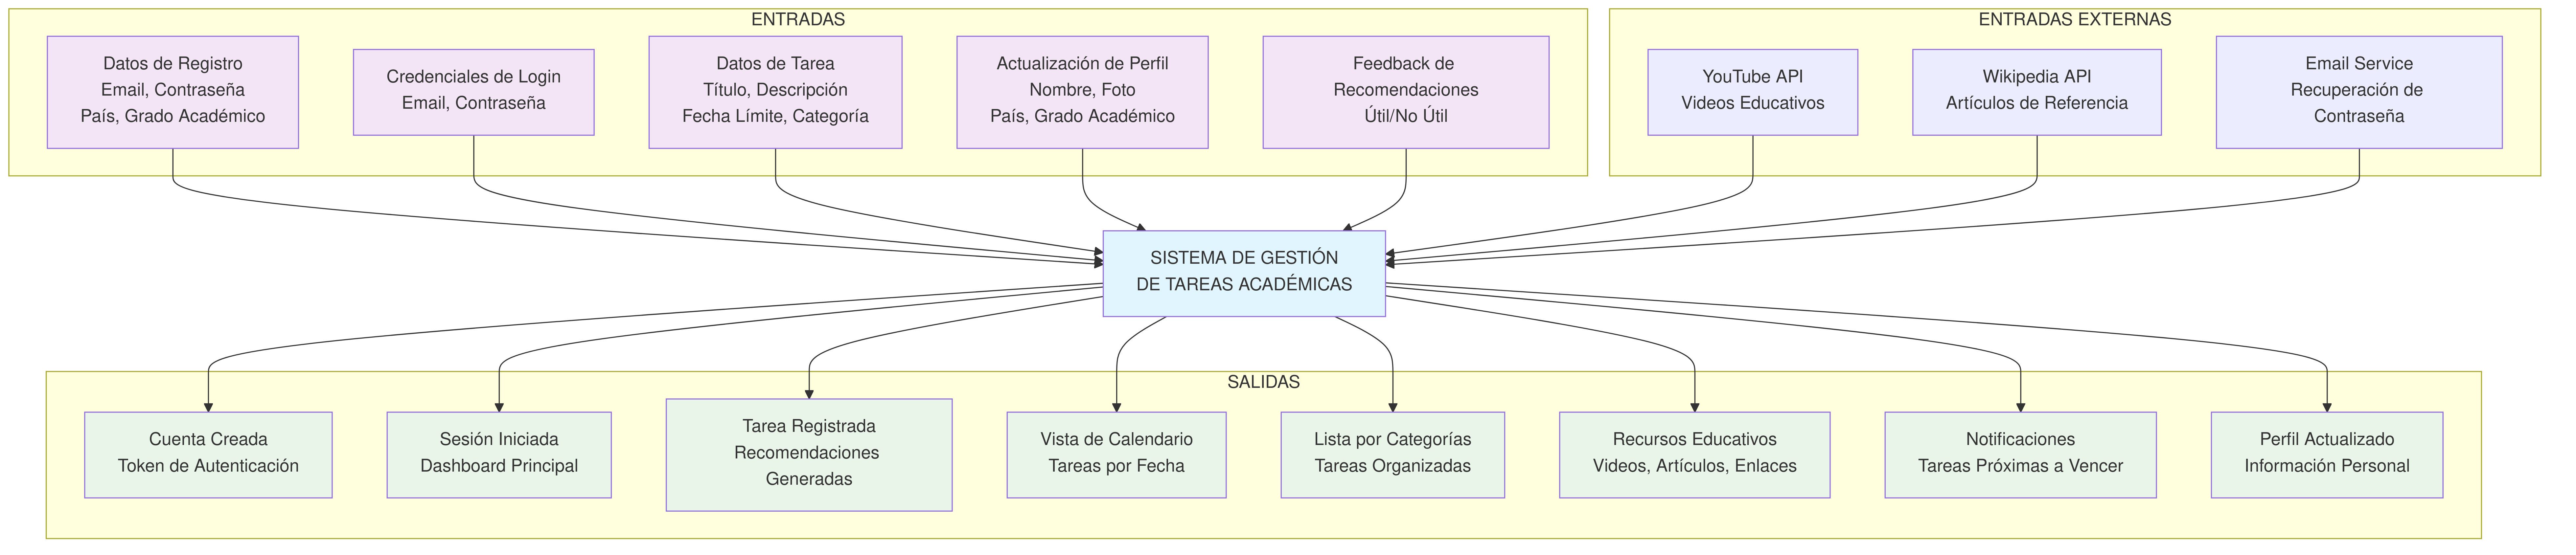
\includegraphics[width=\linewidth]{pngs/e_s.png}
    \caption{Diagrama generado con Mermaid}
\end{figure}

\subsection{Diagrama Entidad-Relación}
\begin{figure}[H]
    \centering
    \includegraphics[width=\linewidth]{pngs/relacional.png}
    \caption{Diagrama generado con Mermaid}
\end{figure}

\subsection{Diagrama de Procesos}
\begin{figure}[H]
    \centering
    \includegraphics[height=\textwidth]{pngs/procesos.png}
    \caption{Diagrama generado con Mermaid}
\end{figure}

\begin{landscape}

\subsection{Diagrama de Casos de Uso}
\begin{figure}[H]
    \centering
    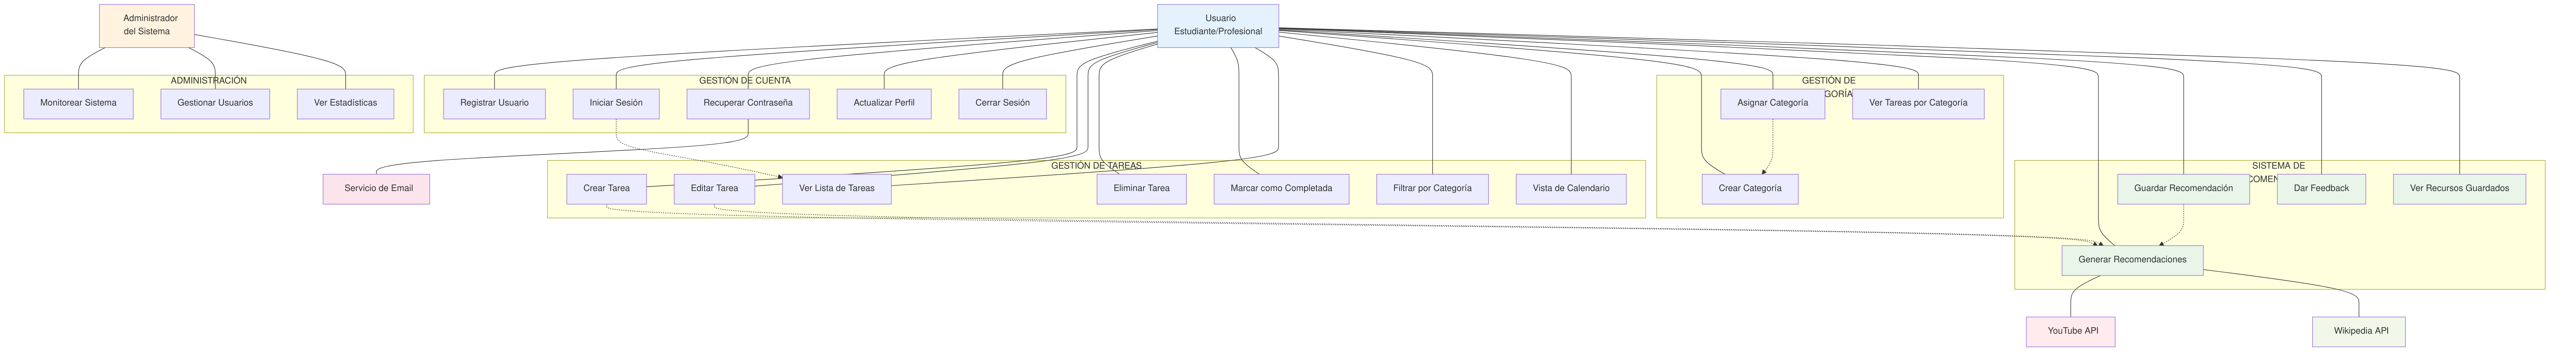
\includegraphics[width=\linewidth]{pngs/use_cases.png}
    \caption{Diagrama generado con Mermaid}
\end{figure}

\subsection{Diagrama de Entradas y Salidas}
\begin{figure}[H]
    \centering
    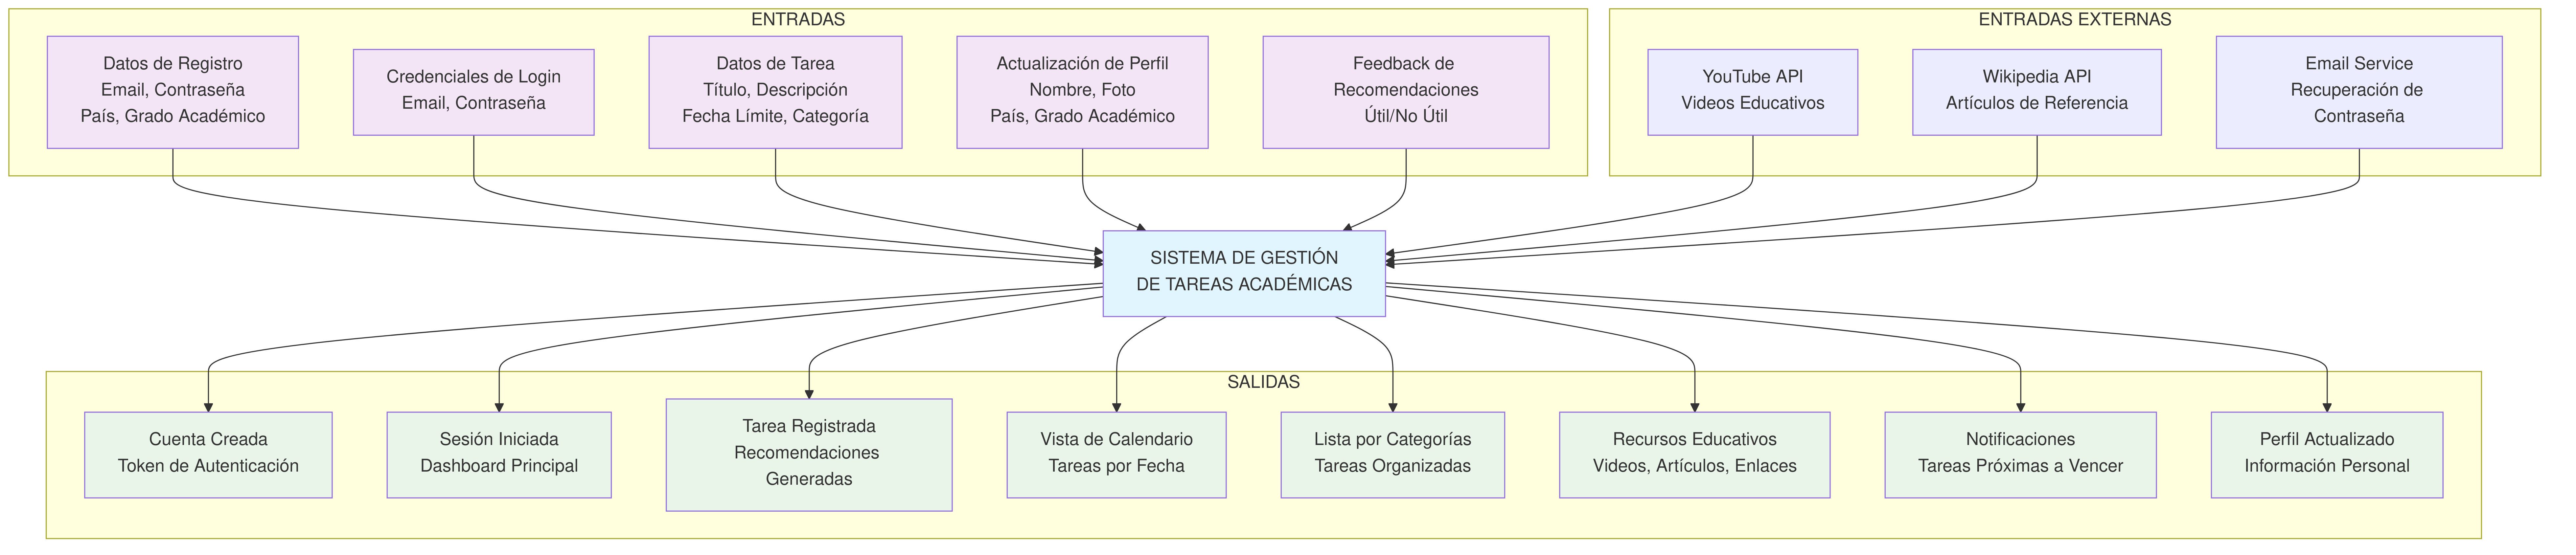
\includegraphics[width=\linewidth]{pngs/e_s.png}
    \caption{Diagrama generado con Mermaid}
\end{figure}

\end{landscape}



%mmdc -i diagramas/nombre_archivo.mmd -o pngs/nombre_archivo.png -b transparent -t default

%%%%%%%%%% BIBLIOGRAFÍA %%%%%%%%%%%%%%%%%%%%%
\pagebreak
\printbibliography[heading=bibintoc]

\end{document}
